\documentclass{article}

\usepackage{adjustbox}
\usepackage{amsfonts}       % blackboard math symbols
\usepackage{amsmath}
% \usepackage{batter_pitcher_2vec}
\usepackage[doi=false,
            eprint=false,
            isbn=false,
            maxbibnames=99,
            sorting=none]{biblatex}        % bibliography
\usepackage{booktabs}       % professional-quality tables
\usepackage[T1]{fontenc}    % use 8-bit T1 fonts
\usepackage{hyperref}       % hyperlinks
\usepackage[utf8]{inputenc} % allow utf-8 input
\usepackage{mathtools}
\usepackage{microtype}      % microtypography
\usepackage{nicefrac}       % compact symbols for 1/2, etc.
\pagenumbering{gobble}
\usepackage{subcaption}
\usepackage{tikz}
\usepackage{url}            % simple URL typesetting

\usepackage[margin=0.5in]{geometry}

\begin{document}

\begin{center}
\noindent{\texttt{(batter|pitcher)2vec}: Statistic-Free Talent Modeling With Neural Player Embeddings}

\noindent{Michael A. Alcorn}
\end{center}

Baseball is notorious for its culture of statistical bookkeeping. The depth and breadth of baseball statistics allows fans and professionals alike to compare players and forecast outcomes with varying degrees of accuracy. Although many traditional baseball statistics can be quite informative and useful, they can also be somewhat arbitrary, and thus may not accurately reflect the true talent of any given player. The field of Sabermetrics was developed in an effort to address some of the inherent limitations of standard baseball statistics. However, many Sabermetrics statistics are similarly ad hoc, reflecting the intuition of the statistic's designer(s). This research introduces \texttt{(batter|pitcher)2vec}, a neural network algorithm that learns to accurately model player talent from ``raw data'', i.e., without resorting to ad hoc statistics.

The task of extracting informative measures of talent for Major League Baseball (MLB) players has a surprising parallel in the field of natural language processing --- the task of constructing useful word embeddings. Words, like MLB players, can be considered distinct elements in a set, and one common way to represent such categorical data in machine learning algorithms is as one-hot encodings. However, one drawback of one-hot encodings is that every element in the set is equally similar (or dissimilar) to every other element in the set (due to their mutual orthogonality). But words (and players) \emph{do} exhibit varying degrees of similarity. By modeling how words behave in different contexts, word embedding algorithms (like \texttt{word2vec}) learn to mathematically encode such similarities as geometric relationships between vectors (e.g., cosine similarity or Euclidean distance). \texttt{(batter|pitcher)2vec} adapts these representation learning concepts to a baseball setting, modeling player talent by learning to predict the outcome of an at-bat given the context of a specific batter and pitcher.

Qualitatively, the learned player representations appear to better reflect baseball intuition than other baseball statistics (Figure~\ref{fig:tsne} and Figure~\ref{fig:batter_traits}) --- for example, by clustering pitchers who rely primarily on pitches with dramatic movement. Further, like \texttt{word2vec}, the representations possess intriguing algebraic properties --- for example, capturing the fact that Bryce Harper might be considered Mike Trout's left-handed dopplegänger. Quantitatively, \texttt{(batter|pitcher)2vec} significantly ($p < 0.001$) outperforms a naïve approach when modeling at-bat outcome probability distributions for previously unseen batter/pitcher matchups. In comparison, a multinomial logistic regression model using identical training and testing data sets (obtained from Retrosheet) performs slightly \emph{worse} than the naïve approach.

These results prove neural embedding algorithms offer a principled means of modeling talent from ``raw data''. Because neural embedding architectures are extremely flexible, they could readily be adapted to a wide variety of sport settings. For example, a neural embedding model that predicts the outcome of a football play could be used to model the ``talent'' of National Football League offenses and defenses. \textbf{495}

\begin{figure}[h]
\centering
\begin{minipage}{.5\textwidth}
\captionsetup[subfigure]{labelformat=empty}
\centering

    \begin{subfigure}[b]{0.75\textwidth}
    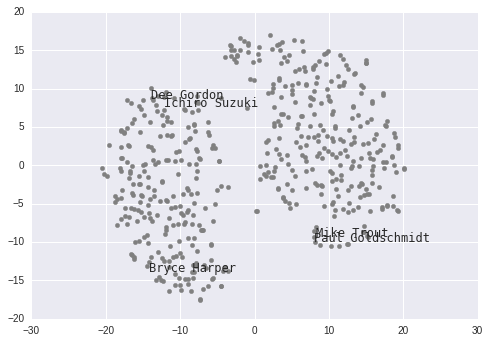
\includegraphics[width=1\linewidth]{batter_tsne.png}
    \caption{}
    \end{subfigure}

    \begin{subfigure}[b]{0.75\textwidth}
    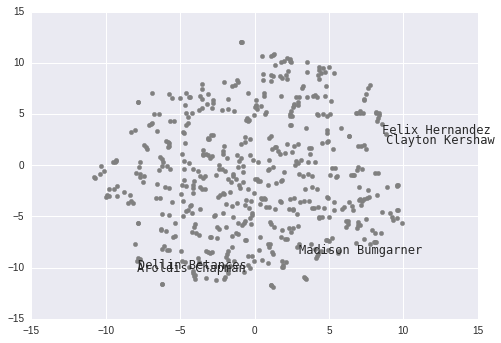
\includegraphics[width=1\linewidth]{pitcher_tsne.png}
    \caption{}
    \end{subfigure}

\caption{Two-dimensional t-SNE map of the learned batter (top) and pitcher (bottom) representations.}
\label{fig:tsne}
\end{minipage}%
\begin{minipage}{.5\textwidth}
\captionsetup[subfigure]{labelformat=empty}
\centering
    \begin{subfigure}{0.5\linewidth}
    \centering
    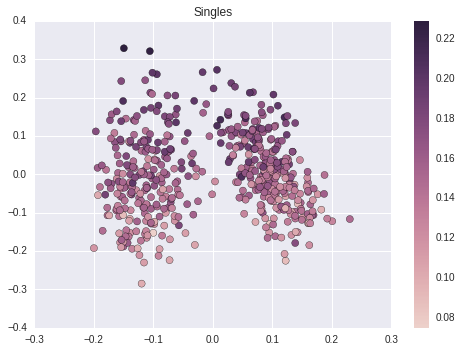
\includegraphics[width=1\linewidth]{batter_single.png}
    \caption{}
    \end{subfigure}%
    \begin{subfigure}{0.5\linewidth}
    \centering
    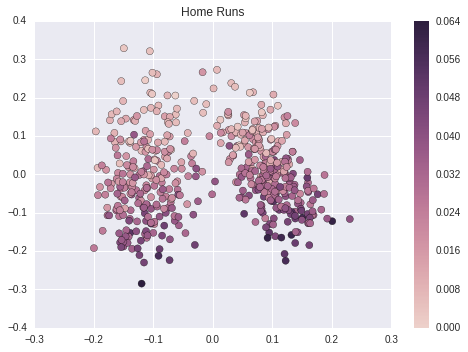
\includegraphics[width=1\linewidth]{batter_hr.png}
    \caption{}
    \end{subfigure}\\[1ex]

    \begin{subfigure}{0.5\linewidth}
    \centering
    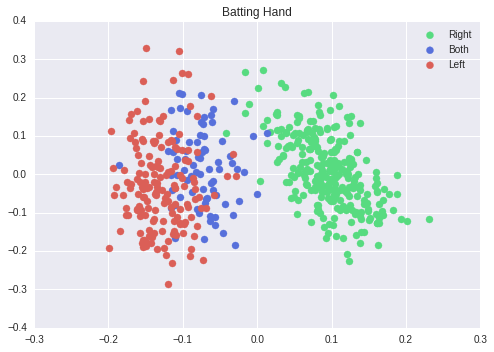
\includegraphics[width=1\linewidth]{batter_hand.png}
    \caption{}
    \end{subfigure}
\caption{Plots of the first two principal components of the batter representations colored by various batter qualities.}
\label{fig:batter_traits}
\end{minipage}
\end{figure}

\end{document}